%-----------------------------------------------------------------------------
\section{Research}\label{sec:research}
%-----------------------------------------------------------------------------
In this document, we have proposed to design a new mathematical and specification subsystem for a mechanical verifier, experiment with the capabilities of a minimalist prover, and apply these to determine the efficacy of specification and mathematical engineering techniques over a library of verified components.

The design of this system will be based on our experience writing and verifying reusable components using the existing RESOLVE verifying compiler, as well as applying lessons from our previous research.

Work on the research proposed in this document will proceed along the path outlined in the introduction, addressing the three points of the problem statement directly in order to test our thesis.

%-----------------------------------------------------------------------------
\subsection{Extensible, Flexible Mathematics for Specification}
%-----------------------------------------------------------------------------
Because every component that is to be verified must be modeled mathematically, the expressiveness of the mathematical system has a direct impact on the facility of the modeling process.  By extension, this impacts the facility of the specification of operations as well, as they must necessarily operate on these mathematical models.  In order to permit components to be modeled and reasoned about at the best level of mathematical abstraction, rather than simply the most convenient, a verification system must permit an extensible mathematical language.  In order to promote the amortization of verification effort over time, the mathematical language must be flexible enough to support patterns of reuse.

Most practical systems do not meet these goals, as their mathematics are limited or built in.  Many pure systems meet them in the mathematical realm, but fail to support the levels of integration with the programmatic realm required to reap the anticipated benefits.  We propose to address this by combining an extensible, flexible mathematical system like those found in pure languages with the modular, reusable techniques of a modern object-based language like those expected for practical systems.

%-----------------------------------------------------------------------------
\subsubsection{Work Completed}
%-----------------------------------------------------------------------------
As we have already published in \cite{bronishMap}, genericity and modularity are crucial attributes of a useful verified component (in that paper, a Map data structure) and systems with inflexible mathematics often sacrifice these attributes by focussing on verifiability alone, yielding verified, but not terribly useful, components.  The mathematical and specification subsystems of our current RESOLVE prototype already contain many features that exemplify the sort of mathematics for verification that we propose.  However, further work is needed to make them extensible and intuitive and to increase the robustness of the implementation.  After much experimentation, described in the various \emph{Work Completed} sections, we have identified the current type system as a major weakness and barrier to extensible, flexible design.  In conjunction with mathematicians here at Clemson and at Ohio State, we have designed a new type system that will be more flexible, more closely match a modern mathematician's conception of the mathematical universe, and, at the same time, be easier to implement because of its regular and reflective nature.

Our new design exploits four key design principles to permit an extensible, flexible system:

%----------------------------------
\paragraph{Higher-Order Logic.}\label{sec:higherOrderDefinitions}
%----------------------------------
If our verified components are to be worth the time we spend verifying them, they must be suitably generic to ensure broad reuse.  Many reuse patterns found in modern programming languages are difficult or impossible to specify or verify using the first-order logic dictated by most practical verification systems and automated provers.  In particular, they make it difficult to apply the lessons of programming to the mathematical world.

Consider, for example the $foldr$ function ubiquitous in functional languages.  $foldr$ takes as its parameters a starting value of type $\gamma$, a function of type $(\gamma*\delta)\rightarrow\gamma$, and a list of elements of type $\delta$.  Starting with the starting value and the first element of the list, the function is applied to yield a new value of type $\gamma$ before repeating the procedure with the resultant value and the next element of the list.  The result of the final function application is returned.  A summing function for lists of integers could thus be defined as:

$sum(zs) = foldr(0, +, zs)$

The broad applicability of such a function for specification should be obvious.  However, even simple theorems describing the mathematical properties of this function run afoul of the first-order restriction that functions may not be quantified over.  For example, Theorem \ref{thm:emptylist} states that $foldr$ applied with an initial value to an empty list simply returns the initial value:

\begin{thm}
$\forall f : (\gamma*\delta)\rightarrow\gamma, \forall ds : List(\delta), (|ds| = 0) \Rightarrow (foldr(i : \gamma, f, ds) = i)$
\label{thm:emptylist}
\end{thm}

Creating definitions that operate on functions is similarly curtailed, preventing development of reusable theories of, for example, transitive functions.

Because our minimalist prover leaves functions and definitions \emph{uninterpretted}, quantifying over them becomes straightforward.  A function or definition is uninterpretted when we do not expand it to consider its definition---i.e., the mathematical subsystem looks at a function or definition variable as a black box, treating it no differently from an ordinary variable.  The tradeoffs inherent in such a design decision are discussed more completely in \cite{tagoreExpand}.

%----------------------------------
\paragraph{First-class Types.}\label{sec:firstClassTypes}
%----------------------------------
First-class types are a feature of several mathematical systems and a handful of experimental programming languages, but were not a part of the original RESOLVE design.  The current prototype treats types as a special case, which makes them difficult and inconsistent to manipulate, limiting the facility of mathematical extension.

The new design incorporates first-class types that are treated as normal mathematical values.  They can be manipulated, passed as parameters, returned as the result of a relation, and quantified over.  This provides both a great deal of flexibilty, as well as a straightforward mechanic for specifying certain generic programming paradigms (most obviously: parameterized type variables.)

For example, the following line would introduce a particular integer called \textbf{1}:

\begin{lstlisting}
Definition 1 : Z = succ(0);
\end{lstlisting}

In exactly the same way, a new type called \textbf{N} could be defined:

\begin{lstlisting}
Definition N : Power(Z) = {n : Z | n >= 0};
\end{lstlisting}

The symbol table maintains information about the kinds of elements that make up any existing class and can thus infer when the symbol introduced by a definition can safely be used as a type.  Thus this is a valid sequence of definitions:

\begin{lstlisting}
Definition N : Power(Z) = {n : Z | n >= 0};
Definition NAcceptor(m : N) : B = true;
\end{lstlisting}

But this one is not:

\begin{lstlisting}
Definition 1 : Z = succ(0);
Definition OneAcceptor(o : 1) : B = true;
\end{lstlisting}

Note that the ``type'' \texttt{Power(Z)} is not actually a type, but rather a function that takes one type and returns another--itself an example of first-class types in action.

Type schemas and dependent types, which define generalized types parameterized by other values, also take advantage of the first-class nature of types and can be defined as normal relations that return a type, rather than using a special syntax.  This requires values that are, in some sense, \emph{of type Type}.  We call this type \textbf{MType} as an abbreviation for \emph{Math Type}\footnote{\texttt{MType} is comparable to * in Haskell, where * is the kind of a type.}.

\begin{sloppypar}
So, as a complete example, consider the String type schema, which represents a finite sequence of elements of a certain type, presupposing the existence of a type \textbf{UntypedStr}, which contains all finite sequences of elements of possibly heterogenous type, and a function called \texttt{Contains\_Only\_Elements\_Of\_Type()} which returns \texttt{true} if and only if a given UntypedStr contains only element of the given type:
\end{sloppypar}

\begin{lstlisting}
Definition Str(T : MType) : MType = 
	{S : UntypedStr | Contains_Only_Elements_Of_Type(S, T)};
\end{lstlisting}

Because they are treated like any other values, such first-class types can be reasoned about by all the same mechanisms already in place for other mathematical values.

%----------------------------------
\paragraph{Mechanisms for Static Reasoning.}\label{sec:staticreasoning}
%----------------------------------
A practical problem with first-class types is the ability to specify types and type-matching situations that are undecidable.  This is an issue common to all systems that permit dependent types--which a system of truly first-class types must necessarily do.

For example we could imagine two types defined by arbitrary predicates:

\begin{lstlisting}
Definition T1 : MType = {E : MType | P(E)};
Definition T2 : MType = {E : MType | Q(E)};
\end{lstlisting}

Determining whether or not an object modeled by \texttt{T1} can be passed where one modeled by \texttt{T2} is expected is equivalent to asking if $\forall e : $\texttt{MType}$, Q(e) \rightarrow P(e)$, which is, of course, undecidable.

Some verification systems (e.g., Coq) take advantage of this very property as an aid to verification, reducing all programs to reasoning about complex types and casting verification as a type-matching problems.  However, because our goal is to permit the use of flexible mathematics on top of a foundation that takes advantage of standard programming models, we would ideally like to provide the usual static type-safety expected by object-oriented programmers.

To this end, we will largely refuse to attempt matching arbitrary mathematical types, relying instead on the programmer or mathematician to provide an explicit mapping in cases where the reasoning is complicated.

In some cases, relationships can be easily inferred.  For example, the case of simple sub-types:

\begin{lstlisting}
Definition Z : MType = ...;
Definition N : Power(Z) = ...;
\end{lstlisting}

Here we can easily note in the symbol table that an \texttt{N} would be acceptable wherever a \texttt{Z} is required and permit such a shift in conception-of-type in certain well-defined cases.

However, hard-coding such relationships does not provide a general mechanism for reasoning about type relationships and with first-class types, we may quickly arrive in situations where we'd expect the ability to reason about complex type relationships without requiring explicit assertions from the programmer or mathematician.  Consider this application of \texttt{Str}s:

\begin{lstlisting}
Definition Average(S : Str(Z)) : Z = ...;
Definition SomeNs : Str(N) = <1, 10, 3, 19>;
Definition AverageOfSomeNs : Z = Average(SomeNs);
\end{lstlisting}

In an ideal world we would expect this to type-check.  But it is not the case that for two general type constructors, if the parameters of the one are subtypes of the parameters for the other, then the results are themselves subtypes.  Consider this (somewhat contrived) complement string type:

\begin{lstlisting}
Definition ComplementStr(T : MType) : MType = 
	{S : UntypedStr | For all i, where 0 <= i < |S|,
		Element_At(S, i) not_in T);
\end{lstlisting}

This is the type of all strings containing possibly-heterogenously-typed elements where no element is of type \texttt{T}.  Clearly, \emph{this} set of definitions should \emph{not} typecheck:

\begin{lstlisting}
Definition Average(S : ComplementStr(Z)) : Z = ...;
Definition NotSomeNs : ComplementStr(N) = <-1, -10, -3, -19>;
Definition AverageOfNotSomeNs : Z = Average(SomeNs);
\end{lstlisting}

However, the same thing that got us into this mess---first-class types---provides a road out.  Because types are normal mathematical values and we already have a mechanism for asserting theorems about mathematical values, we can use that existing mechanism to provide information about type relationships.

Because such theorems must take a specific form if they're to be understood by the static type-checker, we add some special syntax, calling them \texttt{Type Theorem}s instead of ordinary \texttt{Theorem}s.  This flags these theorems for the type checker and ensures that we can raise an error if they do not have the proper form.  So, for example, here is a type theorem stating that, among other things, \texttt{Str(N)}s should be acceptable where \texttt{Str(Z)}s are required:

\begin{lstlisting}
Type Theorem Str_Subtype_Theorem:
	For all T1 : MType, For all T2 : Power(T1),
	For all S : Str(T2),
		S : Str(T1);
\end{lstlisting}

As with any other theorem in the RESOLVE system, this one would require a proof to establish its correctness and maintain soundness.  We assume the presence of a proof-checking subsystem and leave such proofs outside the scope of this research.

Sometimes, more complex relationships are required.  For example, in some circumstances, providing a \texttt{Z} where an \texttt{N} is expected should be fine.  We can use the same mechanism to provide for this case:

\begin{lstlisting}
Type Theorem Z_Superset_of_N:
	For all m : Z, (m >= 0) implies m : N;
\end{lstlisting}

This permits us, under a limited set of circumstances, to provisionally accept a ``sane'' type reassignment, while raising an appropriate proof obligation that the value in question is non-negative.  This is similar to Java, where sane typecasts (i.e., from a \texttt{List} to an \texttt{ArrayList}) are permitted, but cause a run-time check to be compiled into the code.  Here, however, we pay the penalty only once---during verification-time---rather than with each run of the program.

This design splits the difference between a rich, expressive type system and the straightforward static typing programmers have come to expect.  Simple cases can be covered without thought on the part of the programmer, while complex, undecidable cases are permitted by explicitely deferring to the prover.

%----------------------------------
\paragraph{Rich Theory of Mathematical Types.}\label{subsubsect:richSetTheory}
%----------------------------------
When expressing types in a mathematical system, it is natural to look to the Set abstraction.  However, in doing so one must be careful not to inherit any of the many paradoxes and inconsistencies that have dogged the development of theories of sets.  Many schemes exist to correct the deficiencies in naive set theory, with most pure systems using theories based on inductive structures and intuitionistic logics, as these are often well suited to computation.  However, these are quite disjoint from a modern mathematician's conception of the universe.  We choose instead Morse-Kelley Set Theory to be our basis, augmented with higher-order definitions.

First, note that RESOLVE values come in two flavors---mathematical values like the empty set, $\phi$, and programming values like the empty array.  We may trivially show that there are a finite collection of progamming values (after all, there is only a finite number of machine states,) and thus, without loss of generality, we may confine our thinking to the mathematical values, trusting that we can, if nothing else, provide an explicit mapping between the two later.  We thus dispense with distinguishing between them for the moment, using ``value'' to mean ``mathematical value''.

Morse-Kelley Set Theory (MK) defeats Russel's Paradox in the same way as, for example, von Neumann-Bernays-G\"{o}del Set Theory, by imagining that sets are each members of a larger meta-set called the \emph{classes} and admitting the existence of \emph{proper classes}--i.e., set-like objects that are not sets.  We then restrict sets to containing only other sets, while proper classes may contain sets (but nothing may contain a proper class.)  Under this light, we may rephrase the classic example of Russel's Paradox into ``the class of sets that don't contain themselves'', and view its contradiction not as an inconsistency, but rather as a proof that the class in question is proper.

MK permits us all the familiar and natural set constructors, restricted only by the necessity to reason carefully about what classes might be proper.  This is ideal, since mathematicians need not be limited by glaring restrictions to class construction that exist only to eliminate corner-case inconsistencies.  While, in general, only a formal proof can establish a given class as a set, in most cases we can infer it easily as most constructors are closed under the sets---e.g., the union of two sets is always a set.

We will imagine the universe of MK classes to be our universe of types---that is, \texttt{MType} from Section \ref{sec:firstClassTypes}.  Because describing the class that contains all classes would once again introduce Russel's Paradox, we imagine \texttt{MType} is a \emph{meta-class} that exists ``above'' the classes, just as the classes exist ``above'' the sets.

We will imagine that the union of \texttt{MType} with all those things that can be elements of some class to be the universe of RESOLVE values.  We will call this meta-class \texttt{Entity}.  Note that while we may permit \texttt{MType} to be used as part of a type signature, we must be careful not to let it be passed as a parameter---it is not a value.  Though we might permit it to be used informally by imagining that when used as a value it indicates some broad subset of types.

With all this in mind, the RESOLVE mathematical universe can be visualized as in Figure \ref{fig:universe}.

\begin{figure}
  \centering
    \includegraphics[width=.33\textwidth]{universe}
  \caption{A High-level View of the RESOLVE Mathematical Universe\label{fig:universe}}
\end{figure}

%-----------------------------------------------------------------------------
\subsubsection{Work To Be Completed}
%-----------------------------------------------------------------------------
The design of the new mathematical and specification subsystem has already been completed at a high level, though work remains to formalize it more completely. In particular, while we believe that the addition of higher-order definitions should not pose any soundness problems since uninterpretted definitions eschew many of the problems related with higher-order theories, this requires more research and theory development to establish.  This said, formally establishing the soundness of the new theory is outside the scope of this research---we seek to demonstrate only the usefulness of this level of abstraction; future work may be required to refine the mathematical details.

Uninterpretted, higher-order definitions have been implemented and well-tested.  The framework for the new type system has been laid and is awaiting the implementation of type theorems before it can be fully implemented and tested.  Once in place, first-class types, the MK set theory, and type theorems will be tested together and refined against a set of target mathematical theories that will be designed to start simple and graduate eventually to the level of complication of generic theories of trees.  While the simpler of these theories have already been developed, the higher-level ones remain.

%-----------------------------------------------------------------------------
\subsection{Minimalist Prover\label{sec:researchProver}}
%-----------------------------------------------------------------------------
At the core of any mechanical verification system is an automated theorem prover responsible for discharging VCs.  By definition, it is the last word on whether or not a particular technique is yielding more or less easily-proved VCs.  As a result of this, most practical systems have focussed on incorporating the latest and greatest provers into their retinue to piggyback on the breakthroughs at the bleeding edge of proving and artificial intelligence and thus increase provability.

While we are happy to support the latest and greatest suite of provers, we hypothesize that in many cases \emph{flexibility} may trump raw performance with respect to mechanically verifying well-engineered software by encouraging good specification and mathematical engineering that captures the programmer's intuition rather than compromising to work within the framework of a target prover.

In order to experiment with this hypothesis and identify those prover capabilities and performance tunings required to verify well-engineered software, we set out to create a \emph{minimalist automated prover}, starting with only the bare essential capabilities and expanding only when a significant number of VCs appeared that could not be addressed with the prover as it stood.  The result of this effort was RESOLVE's integrated rewrite prover.  As we've refined our design, it has become a platform for prover experimentation within the group and we intend to use it as the yardstick against which to measure our success using our new mathematical system to verify components.

%-----------------------------------------------------------------------------
\subsubsection{Work Completed}
%-----------------------------------------------------------------------------
In \cite{smith10}, we present our architecture for an extensible platform for minimalistic prover experimentation.  The implementation of this prover is in a working form and has been used for several years as part of the RESOLVE toolchain, incuding as part of our education effort centered around the RESOLVE integrated web development environment\cite{chuckThesis}.  This prover has been used in support of a number of our verification publications, including \cite{Sit11} and \cite{smithMinimalist}.  We see the results of a successful verification from the web interface in Figure \ref{fig:successfulverification}.  This is a verification of a realization of the \texttt{Flip()} operation introduced in Section \ref{sec:resolveBackground}.  Enhancement realizations often involve a small number of mathematical types (in this case, almost entirely Strings) and are therefore more straightforward to verify.  Data structure realizations, on the other hand, often have to map from one representation to another, introducing many related types.  As a result, while we can prove them by hand, the mechanical verification of data structures is consigned to Work to be Completed.

\begin{figure}
  \centering
    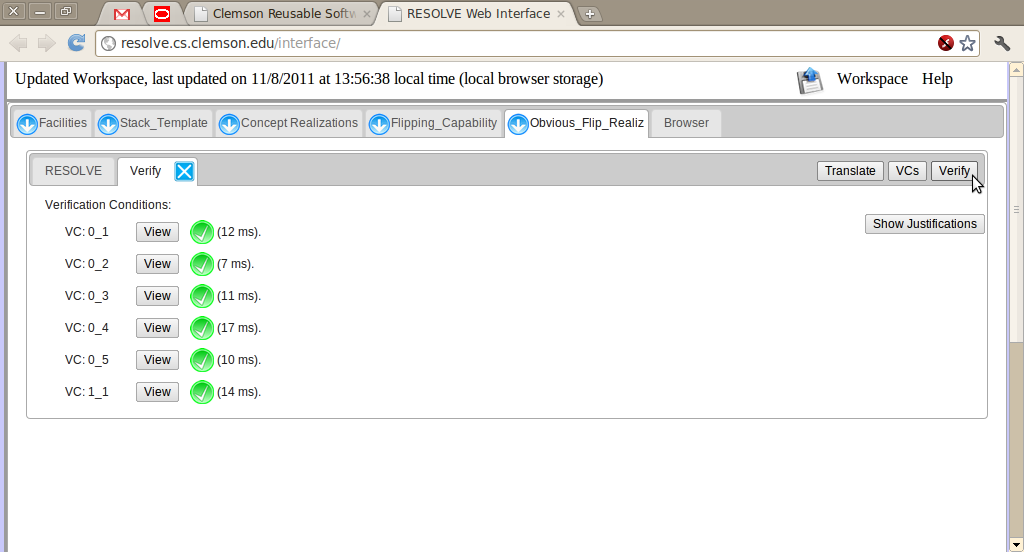
\includegraphics[width=\textwidth]{successfulverification}
  \caption{Our Minimalist Prover at Work\label{fig:successfulverification}}
\end{figure}

As part of our experimentation to-date, we have utilized the extensible plug-in architecture of the prover to add a number of capabilities.  These have included heuristics to make intelligent theorem choices based on the VC at hand, a graphical front-end that permits the user to guide the prover, and a number of preprocessing options to simplify and normalize incoming VCs.  In \cite{smithMinimalist} we perform a comparison of proof complexity (in terms of number of proof steps, including backtracks, taken before reaching a complete proof) based on a simple component using a number of different feature configurations.  This exploration was very illuminating as to which features gave good results.

%-----------------------------------------------------------------------------
\subsubsection{Work To Be Completed}
%-----------------------------------------------------------------------------
With the harness already in working order, the most important addition is that of facilities for mechanically characterizing VCs according to a number of different mechanisms.  Our current depth-first search is more efficient than a breadth-first search, but means that we do not necessarily find the \emph{shortest} proof.  Work is needed to permit a breadth first option when we're willing to trade some efficiency for a more precise metrics.  In addition, we imagine some metrics will be related to the theorems used and the current prover output takes the form of a plain-text ASCII dump, which is not ideal for processing.  A better solution must be engineered so that proofs can be compared and processed mechanically.

Additionally, we would like to expand our efforts to collect data on different prover feature configurations by applying this analysis to a broader range of components.  As mentioned in the Work Completed section, we are eager to expand mechanical verification from enhancement realizations to data structure realizations.  This process will include the explorations of features that have yet to be identified and may be included upon discovering their usefulness for practical VCs.  As an example of a capability we have identified but have yet to implement, we consider a snippet from a realization of a \texttt{Merge\_Sort()} enhancement for queues.  As part of a loop invariant we state:

\texttt{Is\_Permutation(\#Q o \#R, Merger o <Q\_Min> o Q o R)}

Clearly, in the context of a permutation, the concatenation operator is commutative.  Unfortunately, any straightforward commutativity theorem requires us to play a complicated shell game to rearrange arbitrary chains of concatenation.  We could use a torrent of theorems to try and cover all cases, but we suspect that at that point, we have followed minimalism to a ridiculous extreme.  We would like, instead, to permit such context-sensitive properties to be stated in a general way, after which a better internal prover representation than a tree could be chosen to better reflect the properties of the conjunct.

We would also like to experiment with minimalistic proving algorithms.  For example, in addition to the back-tracking, depth- or breadth-first search algorithm we establish in \cite{smith10}, we could imagine that we instead start with our set of antecedents and our set of consequents, then transitively build up a larger and larger set of known antecedents as we simultaneously build up a set of possible justifications for each conjunct of the consequents, dispatch a conjunct whenever its justification set intersects the antecedent set. 

Finally, the prover will need to be adapted to work with the new mathematical type-system, though this modification should be straight-forward since complex reasoning about types is unnecessary in the prover, which need only be able to answer the questions ``What is the type of this expression?'' and ``Does an expression of this type bind to this free variable?''  The former question ought to be answered before the prover is ever invoked, while the latter should be a straightforward library call to the symbol table.

%-----------------------------------------------------------------------------
\subsection{Specification and Mathematical Engineering}
%-----------------------------------------------------------------------------
At its heart the question of specification engineering is one of how equivalent logical expressions affect practical attempts at verification.  As a small example, we may express that a \texttt{Stack}, modelled as a string of \texttt{Entry}s as in Section \ref{sec:resolveBackground}, is empty via $S = \lambda$ or $|S| = 0$.  Indeed, there are an endless number of ways to express this single idea.  In cases where we are largely thinking in terms of contents of the stack, the former may be preferable.  In cases where we are thinking in terms of stack length, the latter may be preferable.  Many current verification systems encourage programmers to state facts many different ways to maximize the liklihood of verification.  We see this as a barrier to usability and would instead like to suggest best practices so that a fact can be stated the \emph{most appropriate way}.  In the future, systems might apply an intelligent heuristic converting equivalent expressions as most convenient.

A more complex dimension is the way in which parameter transformations are formed.  In \emph{explicit} style, the final value of each parameter is defined as a relation of inputs, with the variable on the left hand side of an equality and the the function on the right.  In \emph{implicit} style, a relation relates the final value and inputs.  As an example, assuming an operation \texttt{Substring()} that takes a string and a zero-indexed starting and ending index and returns the substring starting at the first index and end going up to but not including the ending index, we might specify \texttt{Pop()} on a \texttt{Stack} this way in explicit style:

\begin{lstlisting}
Operation Pop(replaces E : Entry, updates S : Stack);
   requires S /= empty_string;
   ensures S = Substring(#S, 1, |S|);
\end{lstlisting}

Alternatively, in implicit style:

\begin{lstlisting}
Operation Pop(replaces E : Entry, updates S : Stack);
   requires S /= empty_string;
   ensures #S = <E> o S;
\end{lstlisting}

%-----------------------------------------------------------------------------
\subsubsection{Work Completed}
%-----------------------------------------------------------------------------
We have already begun identifying and experimenting with different dimensions of specification and mathematical flexibility.  In \cite{kirschenbaumDeepMathematics}, we explore the complexity of VCs arising from well-engineered components, reaching the conclusion that the vast majority of them are simple bookkeeping rather deep mathematical results.  We continued this work in \cite{smithSpecificationAbstractions}, classifying VCs resulting from multiple different versions of a specification for the same programmatic component.  We also explored some verifiability metrics to give a more accurate picture of proof difficulty than merely timing the verification attempt.

The metrics introduced in the latter paper were specific to rewrite-style provers (rather than those based on SAT solvers, for which many of these concepts do not apply).  Among them were shortest proof length, i.e., the number of theorems that had to be applied before a successful proof was achieved; and theorem uniqueness, a measure of how specialized or general the required theorems were.

As an example of some recent success with specification engineering, we consider an enhancement operation to sort a queue.  A naive specification involves universal quantifiers and might appear as in Listing \ref{lst:naivesort}.

\lstinputlisting[language=resolve,caption={A Naive Sort Specification\label{lst:naivesort}}]{Naive_Sort.en}

This enhancement is parameterized by a defintion \texttt{LEQV}, which is constrained to have the properties of a total preordering.  The ensures clause of the sorting operation establishes the two important behavioral qualities of a sort: 1) that the elements are in order with respect to the provided operation and 2) that the resulting queue is a permutation of the original.  Note that we must be careful to deal with repeated elements.

Complex as this spec looks, it is exactly of the kind seen almost universally in the verification literature and, to our knowledge, no sorting implementation of general entry types and using a general comparison function is mechanically verifiable.  This is in part because of the difficulty proving mathematical statements involving quantified expressions, as discussed in Section \ref{sec:contributions}.  Because of our hypothesis that eliminating quantifiers would aid in simplifying verification we experimented with rewriting the specification to take advantage of uninterpretted definitions, as in Listing \ref{lst:defsort}.

\lstinputlisting[language=resolve,caption={A Sort Specification with Uninterpretted Definitions\label{lst:defsort}}]{Def_Sort.en}

Notice that we include a theory of string orderings, \texttt{Ordering\_Theory}, which contains a host of useful definitions and theorems.  We now state an equivalent specification that is nonetheless much more succinct and easy to read from the human perspective.  The only definition requiring any explanation at all is \texttt{Is\_Conformal\_With()}, which is a higher order definition that takes a string and a total preordering and returns \emph{true} \textbf{iff} the elements in that string are ordered according to the ordering function.  From the computational side, we exploit the uninterpretted nature of the definitions (i.e., they function only as a black box) to simplify verification.  We do this by providing a set of theorems in \texttt{Ordering\_Theory} for manipulating ordering definition; as, for example, Theorem~\ref{thm:conformal}.

\begin{thm}
\label{thm:conformal}
$\forall T : \mathrm{MType}, \forall S : \mathrm{Str}(T), 
\forall f : (T * T) \rightarrow \mathbb{B}, \forall E : T,\\
\mathrm{Is\_Total\_Preordering}(f) \wedge \mathrm{Is\_Conformal\_With}(S, f) \wedge f(\mathrm{Element\_At}(S, |S| - 1), E) \Rightarrow\\ \mathrm{Is\_Conformal\_With}(S \circ \mathrm{<}E\mathrm{>}, f)$
\end{thm}

Theorems like these may represent deep mathematical results and thus are not automatically provable in general.  In these cases, proofs may be supplied manually and checked mechanically\cite{smith08}.  Note that, unlike proofs of specific programs, proofs of general theorems represents reusable effort.  Such a mechanical proof-checker is assumed to be present for the purposes of this research and is not included in the scope.  

Such a general theory may be called upon repeatedly to simply verification.  In this case, RESOLVE is able to fully and automatically verify an implementation of selection sort against this specification, a feat that, to our knowledge, no other verification system has achieved.

%-----------------------------------------------------------------------------
\subsubsection{Work To Be Completed}
%-----------------------------------------------------------------------------
Conceptual model is only one dimension of mathematical flexibility.  As already mentioned, the mapping of inputs to outputs and choice of equivalent value expressions are others.  No doubt there are more yet to be clearly identified.

We would like to expand on the experimentation we've already done by creating addional components of a variety of kinds and then specifying them in ways that span the dimensions we've identified.  One source for such components is our previously published set of verification benchmarks\cite{Benchmarks}, which include a number of challenges ranging from toy examples to data structures to complex manipulations.

Once created, we can set our prover to verifying these components and collecting data in an attempt to identify patterns in the ease of verification (or lack there of) under different kinds of specification and mathematical expression and their various interactions.
